\chapter{Introduction}
\label{chap:introduction}

Entre l'identification d'une cible thérapeutique et la mise sur la marché d'un nouveau médicament, une dizaine d'années de recherche et plus d'un milliard d’euros sont nécessaires\cite{DiMasi_price_2003, Siddiqui_high_2012} (voir figure \ref{fig:entonnoir_drug_design}). Afin d'accélérer ce processus et ainsi d'en diminuer le coût, les simulations informatiques sont massivement utilisées. Pour s'approcher au maximum des conditions réelles, et donc de ce qu'il se passe dans le corps humain, ces simulations doivent avoir lieux dans l'eau, c'est à dire en solution. Malgré la puissance de calcul des ordinateurs actuels, ces simulations restent limitées à cause du nombre important de molécules d'eau nécessaires. Afin de s'adapter au mieux aux besoins des différentes études, il existe plusieurs représentations du solvant qui permettent de choisir entre vitesse et précision. Dans ce manuscrit, nous allons présenter la théorie de la fonctionnelle de la densité moléculaire (MDFT) qui allie vitesse et précision. Mon projet de thèse consiste à effectuer le premier pas vers toutes ces applications en adaptant la théorie ainsi que son implémentation aux systèmes biologiques.

\begin{figure}[h]
  \center
  \begin{tikzpicture}

    \draw[fill=white!30!yellow] (0,1,0)--(3,3,0)--(3,9,0)--(0,11,0)--cycle;
    \draw[fill=white!30!orange] (3,3,0)--(6,4.5,0)--(6,7.5,0)--(3,9,0)--cycle;
    \draw[fill=white!30!red] (6,4.5,0)--(12,5.5,0)--(12,6.5,0)--(6,7.5,0)--cycle;


    \draw (-1.5,6) node[above]{\textasciitilde M} ;
    \draw (-1.5,6) node[below]{composés} ;
    \draw (1.5,6) node[above]{\textasciitilde 10K} ;
    \draw (1.5,6) node[below]{composés} ;
    \draw (4.5,6) node[above]{\textasciitilde 250} ;
    \draw (4.5,6) node[below]{composés} ;
    \draw (9,6) node[above]{\textasciitilde 5} ;
    \draw (9,6) node[below]{composés} ;
    
    \draw (1.5,11.5) node[above]{recherche et} ;
    \draw (1.5,11.5) node[below]{découverte} ;
    \draw (4.5,9.5) node[above]{développement} ;
    \draw (4.5,9.5) node[below]{pré clinique} ;
    \draw (9,8) node[above]{essais} ;
    \draw (9,8) node[below]{cliniques} ;

     \draw[fill=red]  (14.5,6,0) circle (0.3);
     \draw[red, fill=red] (14.5,6.3,0)--(14,6.3,0)--(14,5.7,0)--(14.5,5.7,0)--cycle;
  	 \draw[fill=red] (14.5,6.3,0)--(14,6.3,0)--(14,5.7,0)--(14.5,5.7,0);
     \draw[fill=white] (13.5,6,0) circle (0.3);
     \draw[white, fill=white] (13.5,6.3,0)--(14,6.3,0)--(14,5.7,0)--(13.5,5.7,0)--cycle;
     \draw[fill=white] (13.5,6.3,0)--(14,6.3,0)--(14,5.7,0)--(13.5,5.7,0);

     \draw[line width=2pt, latex-latex] (0,0) -- (3,0);
     \draw[line width=2pt, latex-latex] (3,0) -- (6,0);
     \draw[line width=2pt, latex-latex] (6,0) -- (12,0);

    \draw (1.5,0) node[below]{3 années} ;
    \draw (4.5,0) node[below]{1-2 années} ;
    \draw (9,0) node[below]{6-7 années} ;

  \end{tikzpicture}
    \caption{XXXXXXXXXX}
    \label{fig:entonnoir_drug_design}
\end{figure}

\section{Contexte}
Avant d'envisager le développement d'une nouvelle solution thérapeutique il est nécessaire de comprendre les phénomènes à l'origine de la maladie que l'on souhaite guérir. La première étape consiste donc à comprendre la cascade biologique à l'origine de cette maladie. Une fois le phénomène identifié, les chercheurs vont sélectionner une protéine impliquée dans cette cascade. Cette molécule sera appelée "cible". A partir de cet instant, le développement d'un médicament va consister à trouver  parmi plusieurs millions de petits composés le meilleur candidat avant de l'optimiser. Ce candidat doit répondre à plusieurs critères: il doit (i) pouvoir accéder en quantité suffisante à la protéine cible, (ii) se lier à elle et l'inhiber afin de bloquer la cascade biologique à l'origine de la maladie visée et (iii) se lier le moins possible à d'autres protéines afin de minimiser les effets secondaires. Pour des raisons de sécurité, de temps et de coût, il est bien sur impossible de tester l'ensemble de ces millions de molécules en laboratoire ou en essai clinique. Les simulations informatiques sont donc massivement utilisées afin d'effectuer un premier tri et de passer de plusieurs millions de candidats à seulement quelques milliers. Les candidats ayant passés avec succès les différents tests (toxicité, affinité avec la cible, ...) seront ensuite synthétisés et testés en laboratoire. Une poignée de molécules prometteuses sera enfin testée en essai clinique. C'est seulement à l'issu de ce processus long et coûteux qu'une molécule pourra devenir un médicament. Tous ces phénomènes se déroulent dans le corps humain et donc en solution, le solvant aura donc un rôle clé dans l'ensemble de ces processus.



\section{Solvatation}
La solvatation est le phénomène chimique qui consiste à plonger un composé, le soluté, qu'il soit solide, liquide ou gazeux en solution. Une fois en solution, la stabilité ainsi que le rôle du soluté seront fortement influencés par les molécules de solvant\cite{NickPace_protein_2004, levy_water_2004, Meyer_internal_1992, Ladbury_just_1996, GarcaSosa_hydration_2013, Lemieux_how_1996, Tame_role_1996, Li_effect_2005, Snyder_mechanism_2011, Wang_ligand_2011, Mobley_binding_2009, Barillari2007, Olano_hydration_2004, Bren_individual_2012, Ahmed_bound_2011, VAIANA_molecular_2006, Genheden_accurate_2011, Abel_contribution_2011, Biela_ligand_2012, Stegmann_thermodynamic_2009}. Afin de mieux comprendre et analyser cette influence, deux aspects de la solvatation sont étudiés: (i) l'aspect structurale et (ii) l'aspect énergétique. 

\subsection{La structure en solution}
Historiquement, le \textit{drug design} était basé sur la recherche d'une complémentarité de forme entre la cible protéique et le ligand candidat médicament. Cette méthode est appelée \textit{structure-based drug design}\cite{Anderson_process_2003,Zhang_towards_2011,Agrawal_structure_2013}. Dans ce paradigme, la structure de la protéine ainsi que la position des molécules de solvant autour d'elle étaient donc indispensables afin de sélectionner et d'optimiser au mieux les candidats médicament. Devant la quantité croissante de structures disponibles, la \textit{Protein Data Bank}\cite{Bruno_crystallography_2017, Berman_protein_2000} (PDB) à vue le jour en 1971. La PDB est une base de données collaboratives des structures de composés biologiques expérimentalement résolues par RMN\cite{Montelione_recommendations_2013}, rayon X\cite{Read_new_2011} ou encore par microscopie électronique\cite{Henderson_outcome_2012}. A ce jour, plus de 130 000 structures sont disponibles. Cependant, malgré une croissance exponentielle du nombre de structures disponibles, il est récemment apparu que l'étude de la structure ne permettait pas une image complète et précise de ces phénomènes \cite{Henry_structure_2001}. 


\subsection{Les énergies liées à la solvatation}
Le développement récent de calorimètres haute performances permet aujourd'hui d'accéder à une vue énergétique complète de systèmes biologiques\cite{Chaires_Calorimetry_2008, Garbett_thermodynamic_2012, Klebe_applying_2015} et ainsi de venir compléter les données structurales. Il est aujourd'hui par exemple possible, pour une cible donnée, d'acquérir les données énergétiques complètes de plusieurs dizaines de milliers de composés. Parmi les énergies étudiées en drug-design, nous nous intéresserons dans ce rapport aux énergies libres de solvatation ainsi qu'aux énergies libres de liaison.

\subsubsection{L'énergie libre de solvatation}
La première étape nécessaire à tout phénomène en solution est la solvatation. A ce niveau, on considère deux catégories de composés: les composés hydrophiles, qui aiment l'eau (solvophiles pour un solvant arbitraire) et les composés hydrophobes, qui n'aiment pas l'eau (solvophobe pour un solvant arbitraire). Il est possible de différencier ces composées en mesurant expérimentalement ou en prédisant numériquement leurs énergies libres de solvatation. L'énergie libre de solvatation correspond à l'énergie nécessaire au transfert de notre soluté depuis le vide jusqu'en solution. En d'autres termes, sur la figure \ref{fig:solvatation_def}, elle correspond à la différence d'énergie libre entre le système final (soluté en solution) et le système initial (soluté dans le vide + boite d'eau). 

\begin{figure}[h]
  \center
  \begin{tikzpicture}
  \tikzstyle{lien}=[->,>=stealth,rounded corners=5pt,thick]
  \node[inner sep=0pt] (prot) at (0,0)
      {\setlength{\fboxrule}{1pt}%
      {\fbox{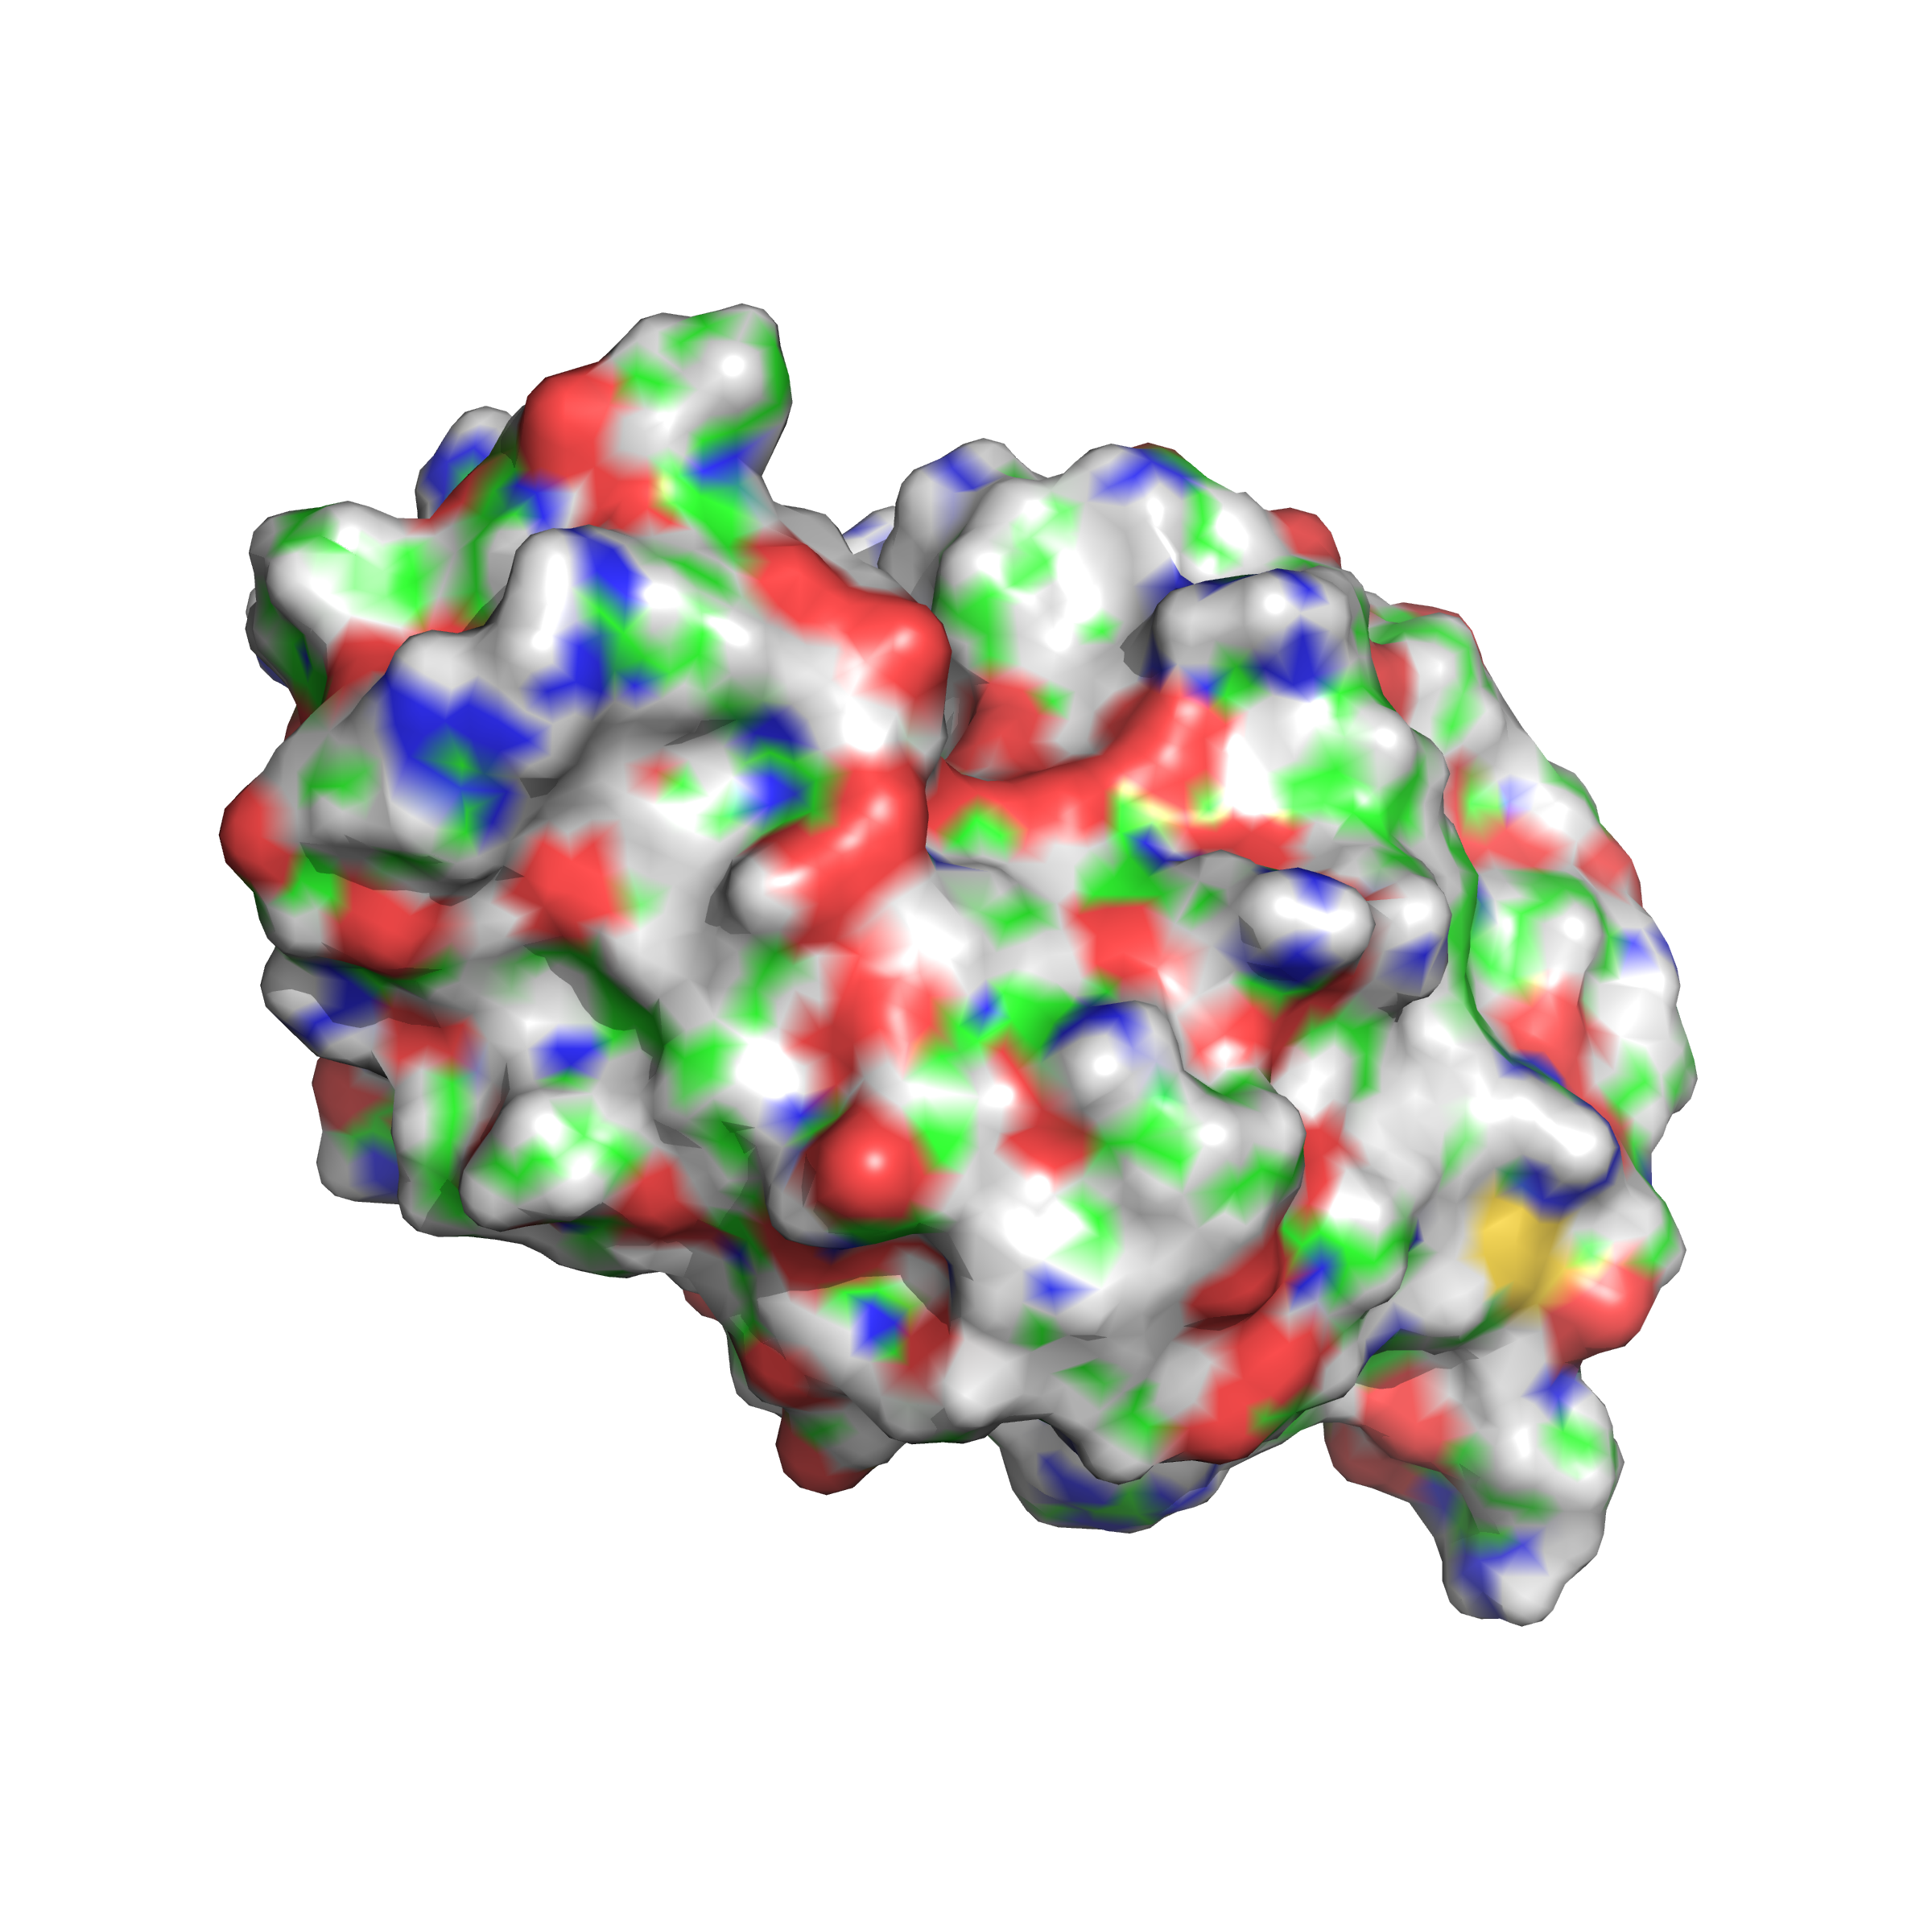
\includegraphics[width=.25\textwidth]{chapters/introduction/images/prot.png}}}%
      };
  \node[inner sep=0pt] (water) at (6,0)
      {\setlength{\fboxrule}{1pt}%
      {\fbox{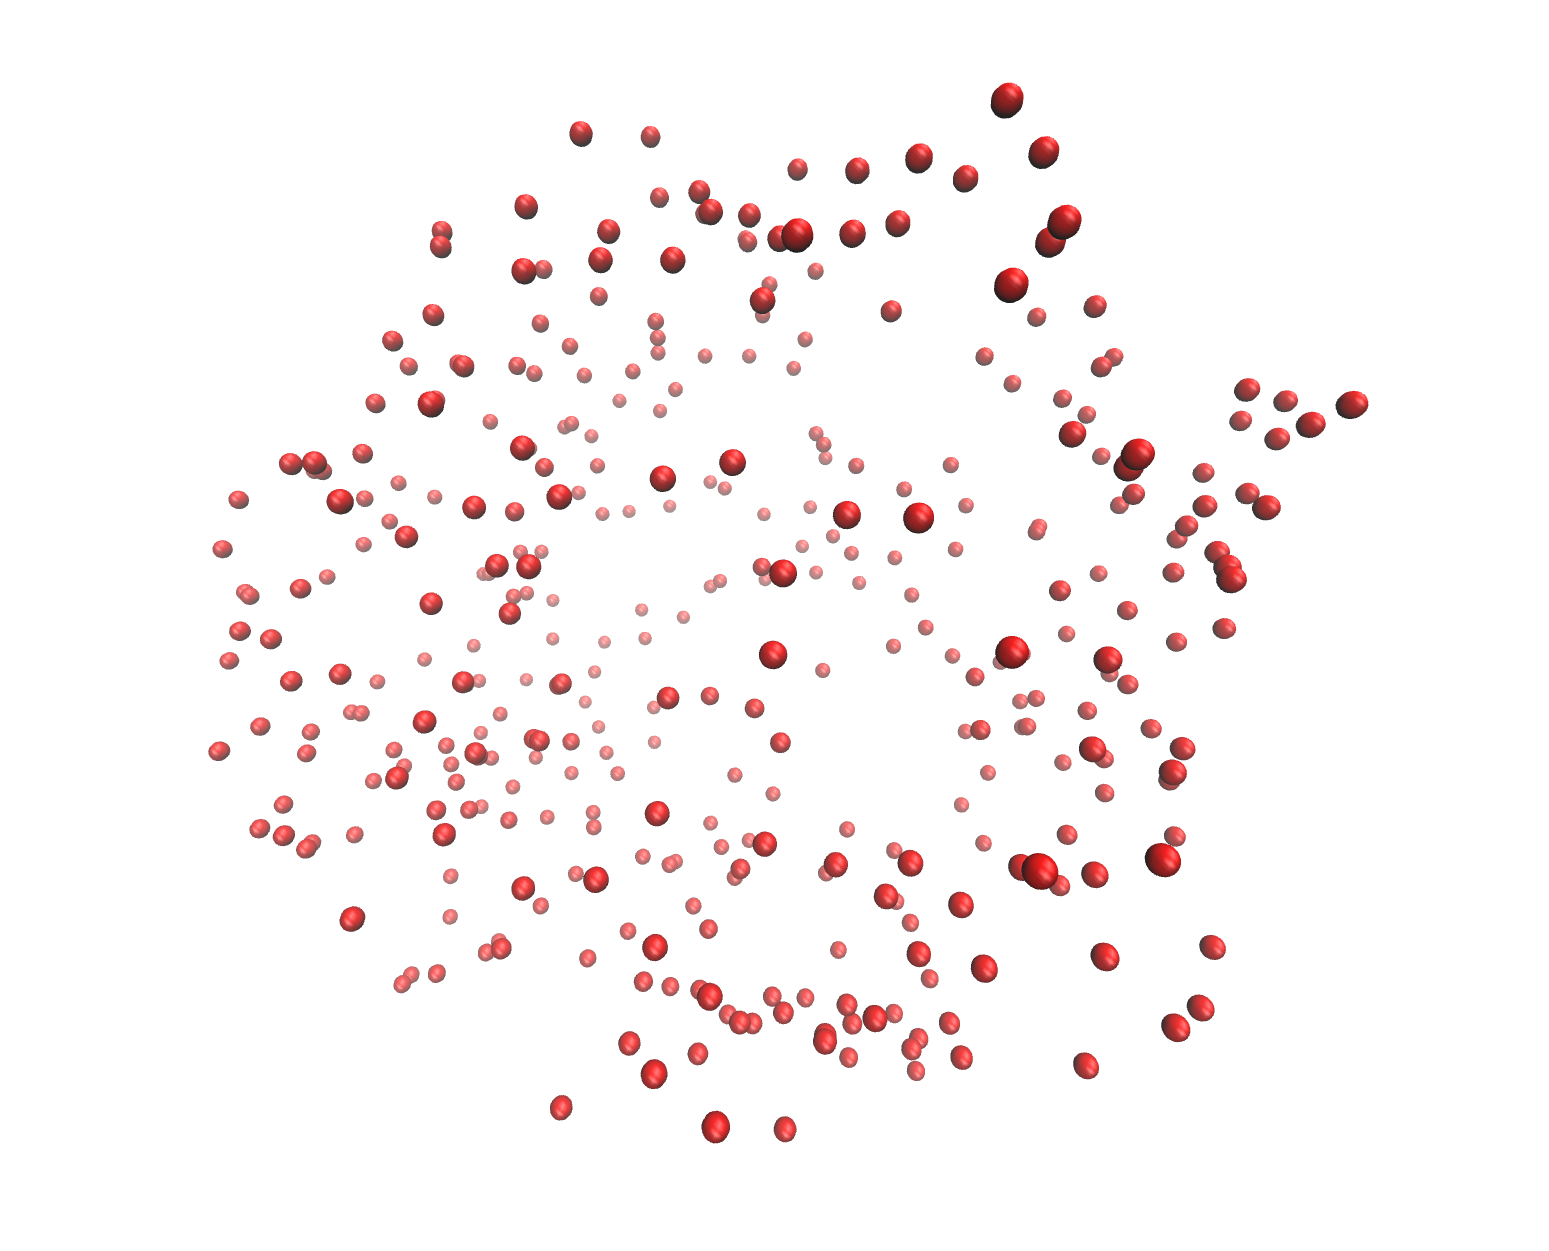
\includegraphics[width=.25\textwidth]{chapters/introduction/images/water.png}}}%
      };
  \node[inner sep=0pt] (prot_water) at (12,0)
      {\setlength{\fboxrule}{1pt}%
      {\fbox{\includegraphics[width=.25\textwidth]{chapters/introduction/images/prot_water.png}}}%
      };

  \draw (2.5,0) node[right] {+};

  \draw[-latex] (water) -- (prot_water);
  
  \end{tikzpicture}
      \caption{Solvatation d'une protéine.}
      \label{fig:solvatation_def}
\end{figure}


La solvation des composés hydrophiles, stabilisés dans l'eau, sera spontanée. Leurs énergies libres de solvatation seront donc négatives. Au contraire, les composés hydrophobes nécessiteront l'apport d'énergie (chauffage, agitation, ...) afin de permettre leur dissolution. Leurs énergies libres de solvatation seront donc positives. 

\subsubsection{L'énergie libre de liaison}
L'énergie libre de liaison correspond à la différence  entre l'énergie libre d'un complexe formé par deux composés comme une protéine cible et un ligand et l'énergie libre de ces deux composés séparés. Pour qu'un médicament soit efficace, il doit se fixer à la protéine cible afin d'en altérer la fonction. Lors de l'optimisation d'un candidat médicament, la valeur la plus faible possible d'énergie libre de liaison sera donc recherchée afin de favoriser l'affinité entre ces deux composés.





\section{Les simulations numériques}
Malgré l'évolution des techniques expérimentales, l'acquisition de données structurelles et énergétiques reste longue et coûteuse. Il n'est donc pas possible de traiter systématiquement l'ensemble des millions de composés disponibles au début du processus de sélection. Les simulations numériques sont donc utilisées pour faire un premier tri. Cependant la façon de considérer le solvant au travers de telles simulations reste un challenge actuel: En effet, par définition, les molécules de solvant sont prépondérantes dans la boite de simulation ce qui fait que la majorité du temps de calcul leur est consacré. Elles représentent donc le facteur limitant de la simulation. Afin de permettre un choix entre précision et rapidité, plusieurs types de représentations ont été proposées pour le solvant\cite{Skyner_review_2015, Reddy_free_2014, brown_free_2010} (voir tableau \ref{tab:temps_calculs}).


\begin{table}[H]
  \centering
  \begin{tabular}{ l | c c | c c }
    \hline & \\[-1em]\hline
    {} & \multicolumn{2}{|c|}{DM/MC} & MDFT & {}\\
    \hline
    Solvant    & explicite & implicite & hybride & {} \\
    \hline
    \multirow{2}{*}{Rapidité}   & \raisebox{-0.3\height}{
\includegraphics[width=0.03\textwidth]{chapters/introduction/images/moins.png}} & \raisebox{-0.3\height}{
\includegraphics[width=0.03\textwidth]{chapters/introduction/images/plus.png}} & \raisebox{-0.3\height}{
\includegraphics[width=0.02\textwidth]{chapters/introduction/images/plus.png}} & {} \\
    {}   & \raisebox{0.3\height}{({\raise.17ex\hbox{$\scriptstyle\mathtt{\sim}$}} jours)} & \raisebox{0.3\height}{({\raise.17ex\hbox{$\scriptstyle\mathtt{\sim}$}} secondes)} & \raisebox{0.3\height}{({\raise.17ex\hbox{$\scriptstyle\mathtt{\sim}$}} minutes)} & {} \\
    \hline
    Précision  & \raisebox{-0.2\height}{
\includegraphics[width=0.03\textwidth]{chapters/introduction/images/plus.png}} & \raisebox{-0.2\height}{
\includegraphics[width=0.03\textwidth]{chapters/introduction/images/moins.png}} & \raisebox{-0.3\height}{
\includegraphics[width=0.02\textwidth]{chapters/introduction/images/plus.png}} & {} \\
    
  \hline \multicolumn{5}{c}{} \\[-1em]\hline
  \end{tabular}
  \caption{Avantage et inconvénients principaux des différents type de solvant utilisés.}
  \label{tab:temps_calculs}  
\end{table}






\subsection{Les méthodes explicites}
Les méthodes explicites représentent chaque molécules de solvant du système. Au prix de temps de calculs importants, ces méthodes sont actuellement les plus précises. Les logiciels de simulation moléculaire de type dynamique moléculaire (MD) ou Monte Carlo (MC), couplées à une représentation explicite du solvant permettent, au prix de temps de calculs longs, d'obtenir avec précision la structure du solvant ainsi que l'énergie libre de solvatation du composé. La structure à l'équilibre du solvant s'obtient à l'issue d'une unique simulation. Elle correspond à la moyenne statistique des positions des atomes de solvant au cours de la simulation XXX PAS BEAU XXX. Plus la simulation est longue, plus l’échantillonnage des conformations est important et meilleure sera la statistique. Une bonne précision nécessite donc une simulation longue et donc un temps de calcul important.

Le calcul de l'énergie libre de solvatation nécessite de coupler les simulations explicites à des méthodes comme l'intégration thermodynamique (TI) ou encore de perturbation d'énergie libre (FEP)\cite{Skyner_review_2015, Hansen_Practical_2014, Christ_basic_2009}. Dans le cas de l'intégration thermodynamique, par exemple, afin de simuler une transition lente de l'état initial à l'état final, une vingtaine de simulations de dynamique moléculaire (MD) ou monte carlo (MC) sont lancées. Chacune d'entre elle représente un état intermédiaire de la transformation étudiée. Une fois l'ensemble des simulations terminées, l'énergie libre de la transformation étudiée correspond à la somme des moyennes de la différence d'énergie potentielle entre deux états voisins. Elle s'écrit sous la forme

\begin{eqnarray}
\Delta F(A \rightarrow B) =  \int_0^1 \left\langle U_B(\lambda) - U_A(\lambda) \right\rangle_{\lambda} d\lambda
\end{eqnarray}

\noindent avec $\lambda$ la coordonnée de réaction permettant la transition entre l'état initial ($\lambda$=0) et l'état initial ($\lambda$=1).
Ces méthodes nécessitant de nombreuses simulations multiplient d'autant le temps de calcul.


\subsection{Les méthodes implicites}
Pour dépasser les limites imposées pas une représentation explicite du solvant, des méthodes rapides, basées sur une représentation implicite du solvant ont été proposées\cite{Skyner_review_2015}. Elles représentent le solvant sous la forme d'un milieu diélectrique continue. Le manque de détails moléculaire comme les liaisons hydrogènes ou la gène stérique ne permet cependant pas un calcul rigoureux des contributions entropiques. Malgré cela, une bonne paramétrisation leur à permis un développement rapide et efficace, avec parfois des prédictions d'énergies libres en bon accord avec les simulations numériques explicites pour des temps de calculs inférieurs de plusieurs ordres de grandeurs. C'est le cas par exemple des méthodes PBSA ou encore GBSA. Ces méthodes très simplifiées fournissent un résultat quasi instantanément. Pour cela, la partie électrostatique est prise en charge en résolvant dans un cas, le modèle de Poisson-Boltzmann résout l'équation de Poisson (PB) et dans l'autre cas le modèle de Born généralisée (GB) résout l'équation du même nom  \cite{Skyner_review_2015}. L'hydrophobicité (la création de la cavité) est quant à elle prise en compte via la surface accessible au solvant (SA). L'énergie libre de solvatation correspond ensuite à une simple combinaison linéaire de ces deux termes.  Ces deux méthodes, couplées à des énergies de mécanique moléculaire, donnent lieux à des méthodes populaires du calcul de l'énergie libre de liaison en solution. Ces méthodes, MM/PBSA\cite{Genheden__MMPBSA_2015} et MM/GBSA seront développées dans le chapitre XXX.

Contrairement aux méthodes explicites, ces méthodes ne fournissent aucune information sur l'organisation du solvant.


\subsection{Les méthodes hybrides}
Les méthodes hybrides, en particulier basées sur la théorie des liquides, constituent une 3$^{ème}$ approche qui allient la vitesse des méthodes implicites à la précision des méthodes explicites. Ces méthodes traitent le solvant sous forme statistique directement à l'équilibre ce qui, contrairement aux méthodes explicites, nous affranchit d'un échantillonnage de l'espace des conformations et permet ainsi un gain de plusieurs ordres de grandeurs en temps de calcul. La première méthode de ce type à avoir été proposée est la théorie des équations intégrales, avec dans un premier temps une représentation atomistique du soluté et du solvant. Les équations intégrales restent cependant difficiles, sensibles aux instabilités numériques et, d'après nos connaissances, limitées aux systèmes en 1 et 2 dimensions à l'exception des développements de Belloni et al.\cite{Puibasset_bridge_2012, belloni_unpublished} qui permettent l'étude de systèmes en quasi 3 dimensions. Ce secteur reste cependant un champ de recherche ouvert. Une approximation de cette méthode à également été développée, le \textit{Reference interaction-site model} RISM, puis dérivée et adaptée aux solutés complexes en 3 dimensions 3DRISM\cite{Chandler_censity_1986,Kovalenko_self_1999}. RISM et 3DRISM ont connue un grand succès car elles permettent de prédire les énergies libre de solvatation et les profils du solvant avec une précision acceptable, comme montré récemment sur des petites molécules neutres, des bio-molécules et même des ions [REF XXX]. Quoi qu'il en soit, ces méthodes considèrent les molécules de solvant comme un ensemble de sites corrélés entre eux, ce qui est schématiquement incorrect.


\subsubsection{La théorie de la fonctionnelle de la densité moléculaire}
La théorie de la fonctionnelle de la densité moléculaire (MDFT) une autre approche de la théorie des liquides. Elle à des connections fortes avec la théorie des équations intégrales, mais est beaucoup moins sensible aux instabilités numériques car elle est basée sur la minimisation d'une fonctionnelle d'un problème variationnel. Le développement d'une fonctionnelle correcte reste cependant difficile et constitue un projet de recherche en cours. La MDFT nous fournit en quelques secondes seulement (quelques minutes pour les plus gros composés), pour des solutés complexes en 3D, deux paramètres essentiels à la compréhension des phénomènes ayant lieu en solution: l'énergie libre de solvatation et le profil de solvatation. Le travail présenté dans ce manuscrit est basé sur cette théorie et son code associé. Le chapitre suivant est dédié à la description de cette théorie.




















\subsection{Quelques exemples}
Ce paragraphe n'a pas vocation à être exhaustif mais simplement à montrer au travers de quelques exemples l'importance de ces paramètres. On considère dans un premier temps la structure du solvant. L'importance de l'eau dans la stabilité et le rôle des protéines n'est plus à démontrer, cette information est donc capitale à la compréhension des mécanismes à l'origine d'une maladie. De la même manière, l'eau en créant un réseau de liaison hydrogènes, aura une influence non négligeable sur l'affinité et donc la stabilité des interactions entre deux composés. Cette information permet donc par exemple d'optimiser un candidat médicament. C'est ce qu'on fait XXX et Al. [REF watermap XXX] dans leur étude. Ils ont calculé l’entropie de chaque molécule d'eau se situant à proximité des interactions. Des fragment ont ensuite été ajoutés à ce ligand (médicament), de façon à venir prendre la place des ces molécules d'eau très énergétiques. En diminuant l'énergie globale du système ils ont ainsi favorisé cette liaison et donc augmenté l'efficacité de ce composé.

L'énergie libre de solvatation peut quant à elle être dérivée en de nombreuses autres grandeurs. Dans les cas des médicaments administrables par voie orale, Lipinski et Al.\cite{Lipinski_lead_2004} ont défini la \textit{régle des 5} qui comporte un ensemble de 4 critères qu'elles doivent respecter. Si une petite molécule ne respecte pas l'ensemble de ces 4 règles, ses chances qu'elles deviennent un jour un médicament oral sont très faibles. Pour respecter ces critères, cette molécule doit posséder au maximum 5 donneurs de liaison hydrogènes, au maximum 10 accepteurs de liaisons hydrogènes, une masse moléculaire inférieure à 550 daltons et un logP inférieur à 5. Si les 3 premiers paramètres peuvent être calculés directement, ce n'est pas le cas du dernier. Le logP correspond au logarithme du rapport entre la solubilité du composé dans l'eau et dans l'octanol. Il peut donc être dérivé des énergies libre de solvatation de ce composé dans ces deux solvants. L'énergie libre de solvatation, couplée à des calculs de mécanique moléculaire permet également de simplifier le calcul de l'énergie libre de liaison. La méthode MM/PBSA\cite{Genheden__MMPBSA_2015} est décrite et dérivée en MM/MDFT dans le chapitre XXX. Enfin on peut citer également le calcul du logBBB (coefficient de partition entre le cerveau et le sang). Dans le cas des maladies neurologiques, le médicament doit pouvoir atteindre le cerveau et donc traverser la barrière hémato-encéphalique. Pour cela, le logBBB doit être compris entre -1 et 0.3\cite{Vilar_prediction_2010}. Ce paramètres peut également être dérivé de la valeur de l'énergie libre de solvatation comme l'on montré Lombardo et al\cite{Lombardo_computation_1996}.

Dans ce paragraphe nous ne présentons qu'une petite partie des possibilités qu'offre une représentation rapide et efficace de la solvatation comme le propose MDFT. Mon projet de thèse consiste à effectuer le premier pas vers toutes ces applications en adaptant la théorie ainsi que son implémentation aux systèmes biologiques.




\vspace{8\baselineskip}

\boitemagique{A retenir}{
Dans ce chapitre nous introduisons le contexte de cette thèse et présentons l'état de l'art des méthodes de solvatation. Nous montrons également en quoi l'énergie libre de solvatation et la structure du solvant sont omniprésentes tout au long du développement et de l'optimisation d'un médicament. 
}



